\documentclass{article}
\usepackage{graphicx} % Required for inserting images
\usepackage{subcaption}

\graphicspath{ {./img/} }

\title{Improving Training Function Performance through Example Filtering}
\author{luca.pepesciarria }
\date{September 2023}

\begin{document}


\maketitle

\section{Introduction}
The training process in machine learning plays a crucial role in model optimization. In this paper, we present a novel approach to improve the performance of the training function by incorporating an example filtering technique. By leveraging the unique characteristics of the hinge loss function, which can yield zero values, we aim to skip examples during each epoch where the loss function evaluates to zero. This filtering mechanism eliminates the need for unnecessary computations during the gradient computation, potentially leading to significant performance improvements.

\section{Methodology}
We describe the mechanism of our proposed example filtering technique, utilizing the hinge loss function. By examining the loss values of individual examples, we identify instances where the hinge loss evaluates to zero. These examples are subsequently skipped during the gradient computation process, since such examples do not incide to the gradient value.

Initially, we implemented our approach using the Flux.jl framework which is optimize for GPUs. However, due to the presence of customized logic in the training process, our approach is not optimal. To mitigate this limitation, we transitioned to SimpleChains.jl, a CPU-optimized alternative that offers better performance on CPU architectures. Nontheless, we start showing how our approach improve the performance on Flux.jl with respect to Flux.jl itself. The improvements is not enough and the use of SimpleChains.jl is required.

For our experiments so far, we used CIFAR10 and MNIST from MlDataset.jl as datasets.

\section{Experimental Evaluation}
We conduct comprehensive experiments to assess the effectiveness of our proposed training function with example filtering. The experiments compare the performance of our algorithm with the base train algorithm. Performance metrics such as loss and accuracy are evaluated to provide a comprehensive analysis. A baseline algorithm incorporating random filtering is used to assess our approach.

\subsection{Running Time}
\begin{figure}[htbp]
    \centering
    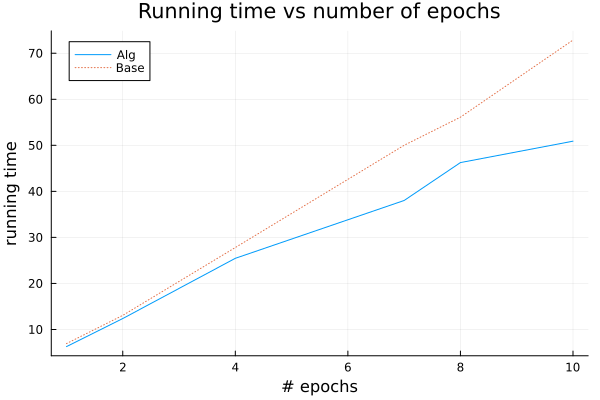
\includegraphics[width=\textwidth]{plot_iter20k.png}
    \caption{Execution Time Comparison of Filtering Algorithm vs. Base Algorithm on 20,000 examples using Flux.jl}
    \label{fig:execution_time_comparison}
\end{figure}

\begin{figure}[htbp]
    \centering
    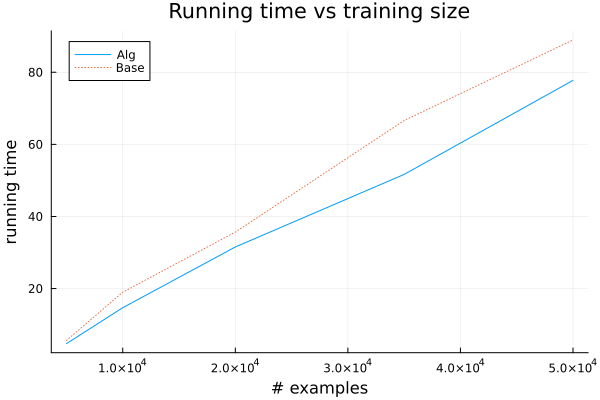
\includegraphics[width=\textwidth]{plot_nexamples.png}
    \caption{Execution Time Comparison of Filtering Algorithm vs. Base Algorithm on different number of examples and 5 epochs using Flux.jl}
    \label{fig:execution_time_examples_comparison}
\end{figure}
 
The plot depicted in Figure \ref{fig:execution_time_comparison} illustrates the execution time comparison between our filtering algorithm and the base algorithm across different numbers of epochs. The x-axis represents the number of epochs, while the y-axis represents the execution time in seconds. The plot demonstrates the superior performance of our proposed filtering algorithm compared to the base algorithm, particularly as the number of epochs increases. The reduced execution time achieved by our approach underscores its efficiency in training machine learning models. These findings substantiate the efficacy of our strategy and its potential impact on accelerating model development and deployment.
The plot in Figure \ref{fig:execution_time_examples_comparison} shows the difference between our filtering strategy and the base training algorithm as the number of examples in the training set increases for a fix number of epochs. Again, the result shows the usefulness of our approach in reducing the running time of the training. 


\begin{figure}[htbp]
    \centering
    \begin{subfigure}[b]{0.3\textwidth}
        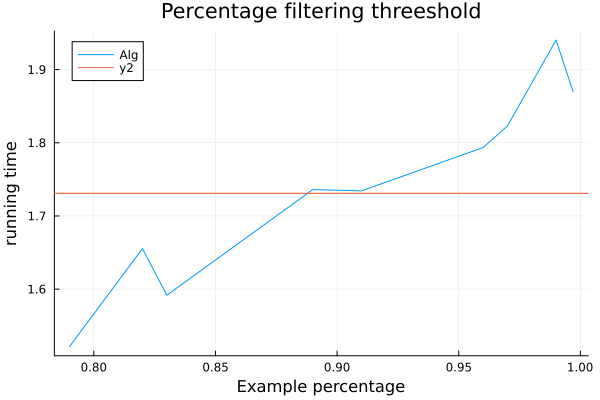
\includegraphics[width=\textwidth]{plot_threeshold1.png}
        \caption{1 epoch}
        \label{fig:threshold1}
    \end{subfigure}
    \hfill
    \begin{subfigure}[b]{0.3\textwidth}
        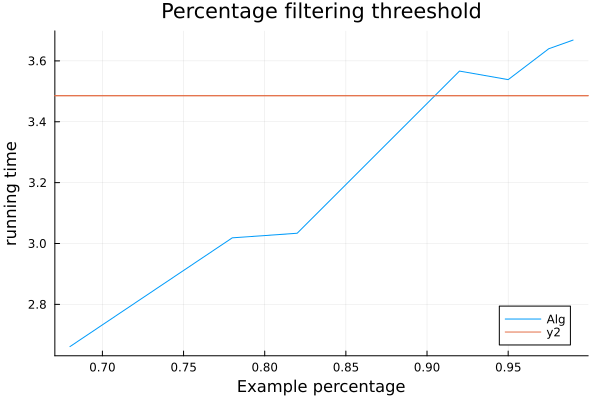
\includegraphics[width=\textwidth]{plot_threeshold2.png}
        \caption{2 epochs}
        \label{fig:threshold2}
    \end{subfigure}
    \hfill
    \begin{subfigure}[b]{0.3\textwidth}
        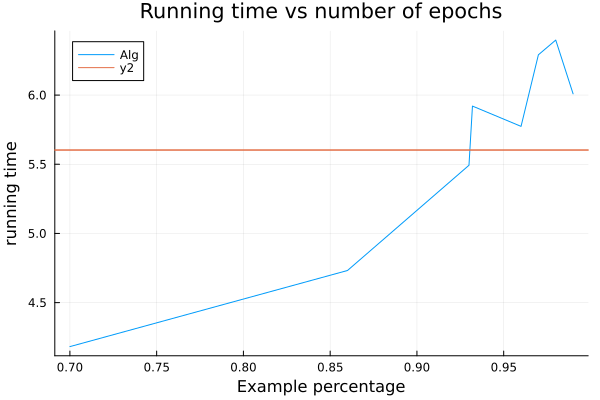
\includegraphics[width=\textwidth]{plot_threeshold3.png}
        \caption{3 epochs}
        \label{fig:threshold3}
    \end{subfigure}
    \caption{Comparison of Execution Time: Percentage of Examples Filtered Out vs. Speed Advantage. The dataset's size is of 5000 examples. In plot b) and c), the percentage refers to the total number of exemples processed (i.e., dataset size times number of epochs).}
    \label{fig:threesholds}
\end{figure}

Next, we switch to SimpleChains.jl. The experiments were conducted to evaluate the performance of our filtering strategy in terms of speed compared to the base algorithm. The objective was to determine the percentage of examples for which our filtering strategy provides a speed advantage. The results showed that if less than 10\% of examples are filtered out, our algorithm is slower than the base algorithm. In other words, if the number of examples used by our algorithm is less than 90\% of the total examples, we achieve faster execution times compared to the base algorithm.

The plots in Figure \ref{fig:threesholds} show the results for increasing number of epochs: 1, 2, and 3.  They illustrate the relationship between the percentage of examples filtered out and the relative speed of our algorithm compared to the base algorithm. The x-axis represents the percentage of examples filtered out, while the y-axis represents the speed advantage or disadvantage of our algorithm relative to the base algorithm.

 When a small percentage of examples, less than 10\%, is filtered out, our algorithm is slower than the base algorithm. This suggests that the overhead introduced by the filtering process outweighs the potential speed benefits gained from reduced data. The number of epochs does not count towards the results of the experiments.

\subsection{Accuracy and Loss}
For what concern the accuracy and loss, as explained before, we tested our approach against the base algorithm and a random filtering strategy. Since the random filtering reduces the dataset's size in the same way our filtering does, their running time is the same. We use that second strategy to investigate how our algorithms performance under accuracy and loss metrics.

The experiments were perform on Flux.jl since SimpleChains.jl performs poorly even in its standard form. On Flux.jl, unfortunately the results show comparable performances between the two filtering strategy and the base algorithm. We think the reason is due to the dataset which is too simple and a small number of example is enough.
\end{document}
